\lab{Algorithms}{Newton-Cotes Integration}{Newton-Cotes Integration}

\objective{Explain Newton-Cotes Integration}

One of the fundamental problems in calculus is integration. However, in the vast majority of cases it is impossible to integrate functions analytically. In these cases our only option is to approximate the integral numerically.

One of the most natural approaches is to use the trapezoidal rule. This approach approximates the integral of a function by using the average of its values at the left and right endpoints of the interval of integration:
\[
\int_a^b f(x) dx \approx (b-a)\frac{f(a) + f(b)}{2}
\]

This approach is equivalent to approximating the integral by integrating the linear interpolant of the function. For an illustration see Figure \ref{Fig:Trapezoidal}

\begin{figure}
\begin{center}
\begin{matlab}
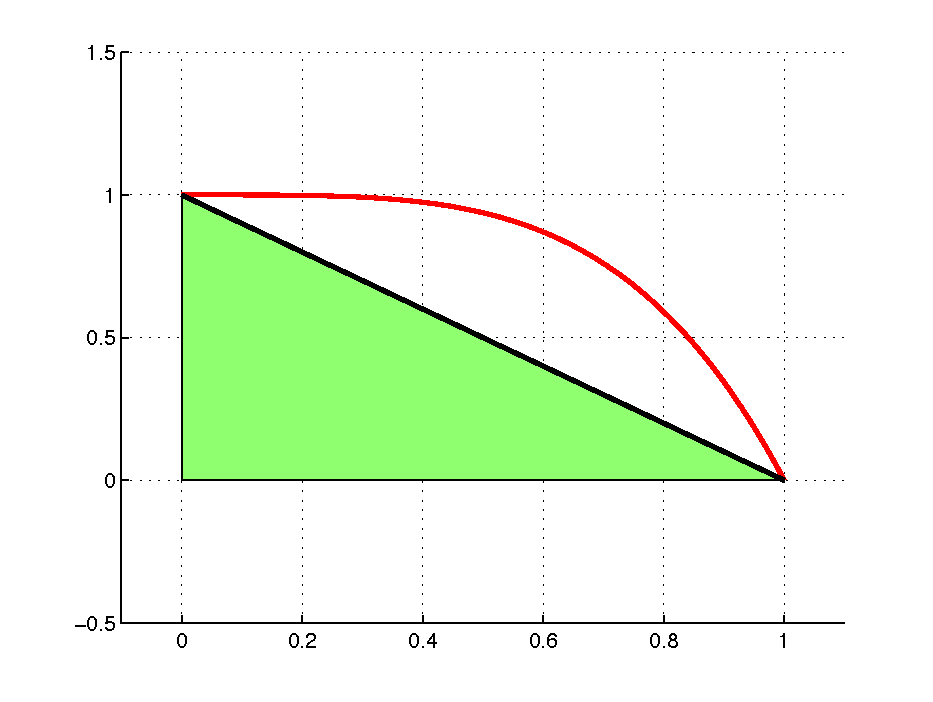
\includegraphics[scale=.3]{./FiguresMAT/Trapezoid.pdf}
\end{matlab}
\begin{python}
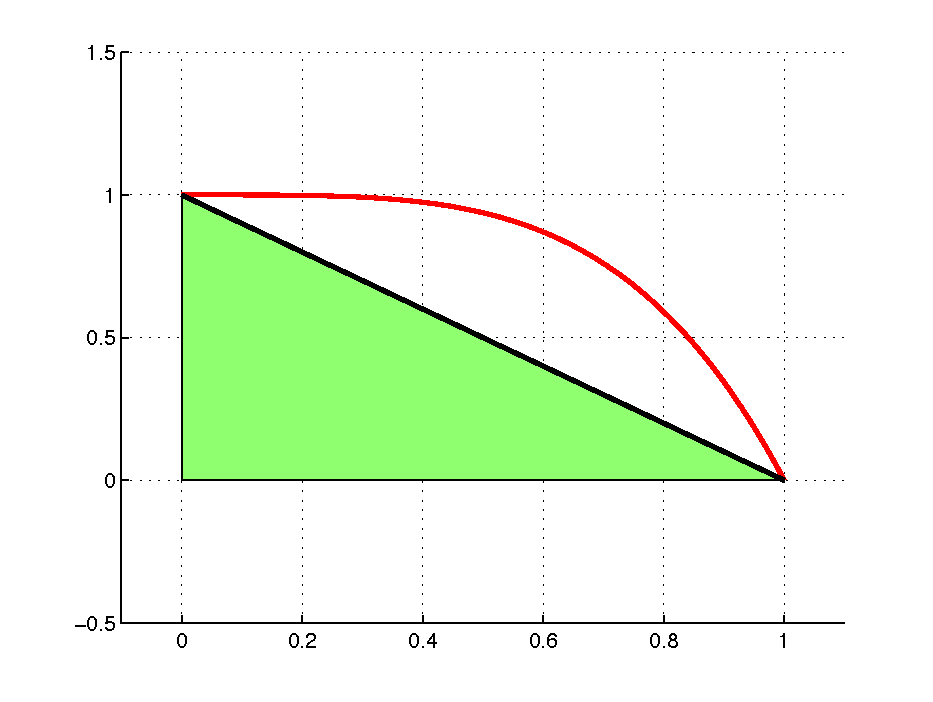
\includegraphics[scale=.3]{./FiguresMAT/Trapezoid.pdf}
\end{python}
\caption{Demonstration of approximating the integral $\int_0^1 (1-x^4)dx$ using the trapezoidal rule. The shaded area is the area approximated by the trapezoidal rule, and the actual function is given in red.}
\label{Fig:Trapezoidal}
\end{center}
\end{figure}

A few quesions rise naturally about the trapezoidal rule. The first is, how good is our approximation? It turns out, that for a twice differentiable function the error is equal to:
\[
\mbox{ error } = \frac{(b-a)^3}{12}f^{(2)}(\xi)
\]
Where $\xi \in [a,b]$. Thus, the error is proportional to both $(b-a)^3$ and the second derivative. The fact that the error is proportional to the value of the second derivative makes sense: the trapezoidal rule cannot compensate for a function having non-zero second derivative.

How can we more accurately approximate the integral of a function? One technique is to break our interval into many smaller sub-intervals. This is known as a \emph{composite rule}. We will delay discussion of composite rules momentarily and discuss a different approach first.

Note that the trapezoidal rule is really just approximating the integral by integrating the linear interpolant of the function. Suppose instead that we approximate our function with a higher-order interpolant. We can write this method mathematically as follows:
\[
\int_a^b f(x) dx \approx \int_a^b \sum_{j=1}^n L_j(x)f(x_j) dx = \sum_{j=1}^n f(x_j)\int_a^b L_j(x) dx
\]

We can precompute (analytically) the value of $w_j = \int L_j(x)$ for a given set of interpolation points $\{x_j\}$ and thus write our approximation as
\[
\int_a^b f(x) dx \approx \sum_j w_j f(x_j)
\]

A set of points $x_j$ and corresponding weights $w_j$ are known as a \emph{quadrature rule}. In this Lab we will focus on evenly-spaced points $x_j$, and in Lab \ref{Lab:GaussQuad} we will look at other sets of points.

Using three evenly-spaced points we can (using a little algebra) derive the following integration rule:
\[
\int_a^b f(x) dx \approx \frac{(b-a)}{6}\left(f(x_1) + 4 f(x_2) + f(x_3)\right)
\]

This is known as \emph{Simpson's Rule}. \begin{matlab} This is the quadrature rule used in the {\tt quad} function in MATLAB.\end{matlab} We can implement Simpson's rule in \ProgrammingLanguage using the following function:
\begin{matlab}
\begin{lstlisting}[style=matlab]
function out = SimpsonsRule(fun,a,b)
out = ((b-a)/6)*[1 4 1]*fun([a;(b-a)/2;b]);
\end{lstlisting}
\end{matlab}

We can test this function on $sin(x)$ as follows:
\begin{matlab}
\begin{lstlisting}[style=matlab]
>> SimpsonsRule(@sin,0,pi)
ans =
    2.0944
\end{lstlisting}
\end{matlab}

The answer, which we can find analytically, is $2$. For only evaluating the function at three points this is fairly accurate.

{\bf Outline:}
\begin{itemize}
\item Intro: We need a simple, higher-order method for approximating integrals. Here we assume evenly spaced points.
\item The simple approach: naive quadrature, midpoint rule.
\item Higher-order Approximation: Use the Lagrange interpolation
\item This yields weights that are fixed for evenly-spaced evaluation points, that are still higher-order approximations
\item Problem: At very high orders, with evenly-spaced points, we get Runge's phenomenon.
\end{itemize}

\begin{problem}
Derive Simpson's Rule. Code and use. Note exactness for lower order polynomials.
\end{problem}

\begin{problem}
Develop Higher Order generator. Simpson's 3-8 Rule
\end{problem}

\begin{problem}
Demonstrate Runge's phenomenon. Explain how to use a composite rule to overcome this.
\end{problem}
